%!TEX program = xelatex 
\documentclass[a4paper,12pt]{article}
\usepackage{fontspec}\defaultfontfeatures{Ligatures=TeX}
\usepackage[a4paper,vmargin={3cm,3.5cm},hmargin={3cm,3cm}]{geometry}
%-----------------------------------------------------------------------------%
\usepackage{settings}
%-----------------------------------------------------------------------------%
%%% Title %%%
\title{G6411 Recitation Notes: Hypothesis Testing: Trinity}
\author{Jesse Chieh Chen\\\href{mailto:cc5229@columbia.edu}{cc5229@columbia.edu}}
\date{\today}
%-----------------------------------------------------------------------------%

\begin{document}

\maketitle

\section{The Holy Trinity of Hypothesis Testing}

Suppose that $\theta\in\Theta\subseteq\reals^k$ and we want to test
\begin{align}
	H_0:r(\theta)=0
	\qquad\text{against}\qquad
	H_1:r(\theta)\ne0,
\end{align}
where $r:\Theta\to\reals^q$ describes $q$ restrictions.
Write $\theta_0$ for the true parameter and
$R(\theta)=\partial r(\theta)/\partial\theta\T$ for the $q\times k$ Jacobian.
We assume that $r$ is continuously differentiable and $R(\theta_0)$ has full row rank.

\begin{remark}[Full Rank]
	Full row rank means that the $q$ restrictions are locally independent.
	For linear restrictions, redundant equations make the Jacobian rank deficient.
	For example, $\theta_1=0$ and $2\theta_1=0$ impose only one independent restriction, since the second equation adds nothing to the first.
\end{remark}

\begin{remark}
	For linear restrictions, we have $r(\beta)=R\beta-r_0$ with $R(\beta)=R$.
\end{remark}

\noindent
The \emph{holy trinity} consists of three approaches:
\begin{enumerate}
	\item \textbf{Wald Test:} Does the unrestricted estimate approximately satisfy the restrictions?
	\item \textbf{\gls{lm} Test:} At the restricted estimate, is there a strong incentive to move away from the null?
	\item \textbf{\gls{lr} Test:} How much does imposing the null reduce the maximized likelihood?
\end{enumerate}
Each measures a different discrepancy between the data and $H_0$.
Under the conditions stated below, all three have a $\chi_q^2$ limiting distribution under the null.
\autoref{thm-trinity} establishes the stronger result that their differences converge to zero under the null:
the three statistics are asymptotically equivalent.

\section{The Wald Test}

Suppose that an estimator $\widehat\theta$ satisfies
\begin{align}
	\sqrt n(\widehat\theta-\theta_0)\dto\normaldistribution(0,V),
	\qquad \widehat V\pto V,
\end{align}
where $V$ is positive definite.
Here $\widehat V$ estimates the variance of the limiting distribution of
$\sqrt n(\widehat\theta-\theta_0)$; the estimated covariance matrix of $\widehat\theta$ is $\widehat V/n$.

\begin{theorem}[Wald Statistic]\label{prop-wald}
	Under $H_0:r(\theta_0)=0$,
	\begin{align}
		T_{\mathrm W}
		\coloneqq n r(\widehat\theta)\T
		\left(R(\widehat\theta)\widehat V R(\widehat\theta)\T\right)\inv
		r(\widehat\theta)
		\dto\chi_q^2.\label{eq-wald}
	\end{align}
	An asymptotic level-$\alpha$ test rejects when $T_{\mathrm W}>\chi^2_{q,1-\alpha}$,
	where $\chi^2_{q,1-\alpha}$ is the $(1-\alpha)$ quantile of $\chi_q^2$.
\end{theorem}
\begin{proof}
	The delta method gives
	\begin{align}
		\sqrt n r(\widehat\theta)
		\dto\normaldistribution\big(0,R(\theta_0)VR(\theta_0)\T\big).
	\end{align}
	Standardizing this $q$-dimensional vector and taking its squared length gives \eqref{eq-wald}.
\end{proof}

\begin{remark}[Interpretation]
	Estimate the unrestricted model, and then measure how far $r(\widehat\theta)$ is from zero relative to its sampling uncertainty.
	It only requires the unrestricted estimate and a consistent covariance estimator.
	In particular, it does not require a correctly specified likelihood: a sandwich covariance estimator can be used.
\end{remark}

\begin{remark}[Linear Restrictions]
	For $H_0:R\theta=r_0$, where $R$ is a fixed $q\times k$ matrix with full row rank and $r_0\in\reals^q$ is a specified nonzero vector,
	we have $r(\theta)=R\theta-r_0$ and $R(\theta)=R$.
	Thus $r(\widehat\theta)=R\widehat\theta-r_0$ exactly, and the Wald statistic becomes
	\begin{align}
		T_{\mathrm W}
		=n(R\widehat\theta-r_0)\T\big[R\widehat V R\T\big]\inv(R\widehat\theta-r_0)
		\dto\chi_q^2\quad\text{under }H_0.
	\end{align}
	No value of $\theta_0$ is needed, and no linearization is involved.
\end{remark}

\begin{remark}[Dependence on Parameterization]
	The Wald test is not generally invariant to nonlinear reparameterization.
	For a positive scalar parameter, the equivalent nulls $\theta=1$ and $\log\theta=0$ give statistics
	$n(\widehat\theta-1)^2/\widehat V$ and $n\widehat\theta^2(\log\widehat\theta)^2/\widehat V$, respectively, using the delta method for the latter.
	These can give different finite-sample decisions, but under the stated regularity conditions they are asymptotically equivalent under the null, with a $\chi_1^2$ limit.
\end{remark}

\begin{example}[Relation to $t$-Statistic]
	For $H_0:\theta_j=\theta_{j0}$, the Wald statistic is
	\begin{align}
		T_{\mathrm W}
		=\frac{n(\widehat\theta_j-\theta_{j0})^2}{\widehat V_{jj}}
		=\left(\frac{\widehat\theta_j-\theta_{j0}}{\operatorname{se}(\widehat\theta_j)}\right)^2.
	\end{align}
	Thus the usual two-sided normal-based test is a one-restriction Wald test.
	Since $Z^2\sim\chi_1^2$ for $Z\sim\normaldistribution(0,1)$,
	$\chi^2_{1,1-\alpha}=z_{1-\alpha/2}^2$ and the two rejection rules agree.
\end{example}

\begin{remark}[Relation to $F$-Test]
	The Wald test can be understood as the scaled asymptotic version of the finite-sample $F$-test in the normal linear model.
	See \autoref{sec-f-test} for details.
\end{remark}

\begin{example}[Applying Delta Method in Practice]
	Suppose $\theta=(\theta_1,\theta_2)\T$ contains two regression coefficients and
	\begin{align}
		\sqrt n(\widehat\theta-\theta_0)\dto\normaldistribution(0,V),
		\qquad \widehat V\pto V,
	\end{align}
	with $V$ positive definite and $\theta_{02}\ne0$.
	We estimate the ratio $\tau_0=\theta_{01}/\theta_{02}$ by $\widehat\tau=\widehat\theta_1/\widehat\theta_2$
	and test $H_0:\tau_0=c$ for a specified constant $c$.
	The restriction and its derivative are
	\begin{align}
		r(\theta)=\frac{\theta_1}{\theta_2}-c,
		\qquad R(\theta)=
		\begin{pmatrix}
			1/\theta_2 & -\theta_1/\theta_2^2
		\end{pmatrix}.
	\end{align}
	The delta method gives
	\begin{align}
		\sqrt n(\widehat\tau-\tau_0)
		&\dto R(\theta_0)\normaldistribution(0,V)
		= \normaldistribution\big(0,R(\theta_0)VR(\theta_0)\T\big).
	\end{align}
	Hence, under $H_0$, we have
	\begin{align}
		T_{\mathrm W}
		= n (\widehat\tau-c)\T \left(R(\widehat\theta)\widehat V R(\widehat\theta)\T\right)\inv (\widehat\tau-c)
		= \frac{(\sqrt{n}(\widehat\tau-c))^2}{R(\widehat\theta)\widehat V R(\widehat\theta)\T}
		\dto\chi_1^2
	\end{align}
	where the asymptotic variance estimator is given by
	\begin{align}
		R(\widehat\theta)\widehat V R(\widehat\theta)\T
		=\frac{\widehat V_{11}}{\widehat\theta_2^2}
		-\frac{2\widehat\theta_1\widehat V_{12}}{\widehat\theta_2^3}
		+\frac{\widehat\theta_1^2\widehat V_{22}}{\widehat\theta_2^4}.
	\end{align}
	The covariance term $\widehat V_{12}$ matters: uncertainty about a ratio depends on how the two coefficient estimates move together.
	The condition $\theta_{02}\ne0$ ensures that the ratio is differentiable at the true parameter.
\end{example}

\begin{figure}[t]
	\centering
	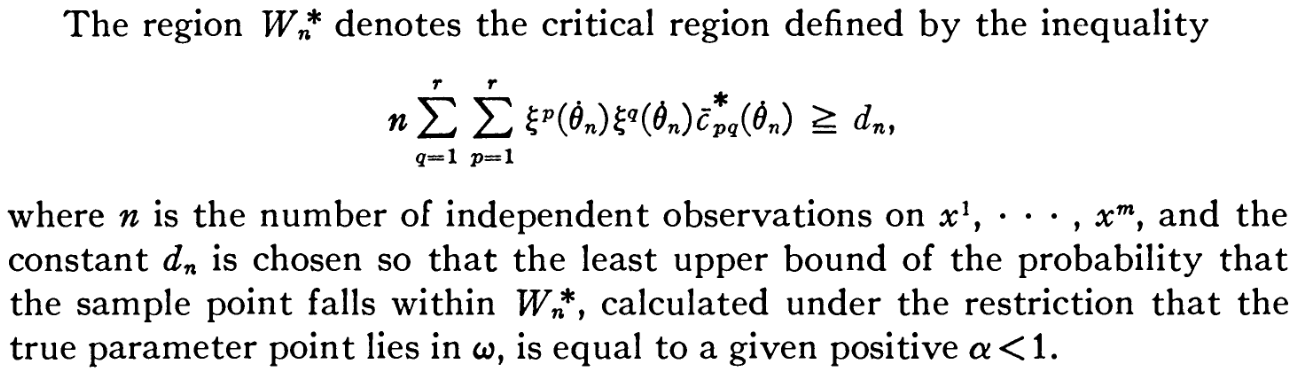
\includegraphics[width=0.75\textwidth]{figures/wald-statistic.png}
	\caption{The original ``Wald test'' in \textcite[481]{wald-1943}.}
	\label{fig-wald-statistic}
	\caption*{\footnotesize%
	\emph{Note}:
	In his notation,
	the parameter vector is $\theta$ and the null hypothesis is $H_0:\xi^{1}(\theta)=\cdots=\xi^{r}(\theta)=0$;
	the estimator is denoted $\dot\theta_n$;
	the $r$-by-$r$ matrix $[\bar c_{pq}^*(\dot\theta_n)]_{p,q}$ is equivalent to our $(R(\widehat\theta)\widehat V R(\widehat\theta)\T)\inv$;
	$d_n$ denotes the critical value;
	$\alpha$ denotes the significance level.
	The quadratic form on the left is the Wald statistic $T_{\mathrm{W}}$ in \eqref{eq-wald}.
	}
\end{figure}

\begin{remark}[Abraham Wald and Columbia University]
	Abraham Wald joined Columbia's faculty in 1941 after fleeing Nazi-controlled Austria.
	During World War II,
	he worked at Columbia's \emph{Statistical Research Group},
	which developed statistical methods for military applications.
	In \citeyear{wald-1943}, he published the first formulation of the Wald test; see \autoref{fig-wald-statistic}.
	After the war, he became chair of the newly formed Department of Mathematical Statistics in 1946,
	the predecessor of today's Department of Statistics.
	He remained at Columbia until his death in a plane crash in 1950.
\end{remark}

\section{Likelihood-Based Tests}

\paragraph{Setup.}

For the next two tests, assume a correctly specified likelihood with parameter $\theta\in\reals^k$.
For \gls{iid} observations, write the \emph{average} log-likelihood as
\begin{align}
	\ell_n(\theta)
	= \frac1n\sum_{i=1}^n \ell_i(\theta)
	= \frac1n\sum_{i=1}^n \log f(Y_i\given X_i, \theta),
	\qquad
	\dot\ell_n(\theta)=\frac{\partial\ell_n(\theta)}{\partial\theta}.
\end{align}
The information per observation is $I(\theta_0) = \E_0 s_i(\theta_0)s_i(\theta_0)\T$
where $s_i(\theta)=\dot\ell_i(\theta)$ and
the expectations average over both $Y_i$ and $X_i$.
The unrestricted and restricted maximum likelihood estimators are
\begin{align}
	\widehat\theta=\arg\max_{\theta\in\Theta}\ell_n(\theta),
	\qquad
	\widetilde\theta=\arg\max_{\theta\in\{\theta:r(\theta)=0\}}\ell_n(\theta).
\end{align}

\begin{remark}[Regularity]
	We work under the usual regularity conditions for \gls{mle}:
	the true parameter is interior, the information is positive definite, the estimators are consistent under $H_0$,
	and the log-likelihood is smooth with its average Hessian converging uniformly near $\theta_0$ to its continuous expectation.
	In particular,
	$\sqrt n(\widehat\theta-\theta_0)\dto\normaldistribution(0,I(\theta_0)\inv)$.
	These conditions exclude redundant restrictions and boundary problems.
\end{remark}

\begin{remark}
	The \gls{lm} and \gls{lr} approaches extend beyond likelihood-based estimation, for example to \gls{gmm}.
	Such extensions require appropriate covariance estimation or weighting.
	Here we use the likelihood formulation to simplify the exposition and connect to the classical literature.
\end{remark}

\subsection{The Lagrange Multiplier Test}

To solve the restricted maximization problem, form the Lagrangian
\begin{align}
	\mathcal L_n(\theta,\lambda)=\ell_n(\theta)-\lambda\T r(\theta)
	\quad\text{with}\quad
	\lambda\in\reals^q.
\end{align}
The restricted estimate and its multipliers solve the first-order conditions
\begin{align}\label{eq-lm-foc}
	\dot\ell_n(\widetilde\theta)-R(\widetilde\theta)\T\widetilde\lambda=0
	\quad\text{with}\quad
	r(\widetilde\theta)=0.
\end{align}
Thus the multipliers determine the average score left at the restricted estimate.
The \gls{lm} test, also called the \emph{score test}, asks whether this remaining slope is unusually large relative to its sampling uncertainty.

\begin{remark}[Interpretation]
	The multipliers measure the marginal gain from relaxing the restrictions.
	If $H_0$ is true, the population objective is already maximized at a parameter satisfying the restrictions,
	so the population multipliers are zero.
\end{remark}

\begin{remark}[Average Score and Multipliers]
	The average score is a $k$-vector, while the multipliers form a $q$-vector.
	The restricted first-order condition relates them by
	\begin{align*}
		\dot\ell_n(\widetilde\theta)=R(\widetilde\theta)\T\widetilde\lambda.
	\end{align*}
	Thus the average score is a linear combination of the restriction gradients, with the multipliers as coefficients.
	Since $R(\widetilde\theta)$ has full row rank, we can also recover the multipliers from the score:
	\begin{align*}
		\widetilde\lambda
		=\big[R(\widetilde\theta)R(\widetilde\theta)\T\big]\inv
		R(\widetilde\theta)\dot\ell_n(\widetilde\theta).
	\end{align*}
	In particular, the average score is zero if and only if all the multipliers are zero.
\end{remark}

\begin{theorem}[Lagrange Multiplier Statistic]\label{thm-lm}
	Let $\widetilde I\pto I(\theta_0)$ be an information estimator computed from the restricted fit.
	Under $H_0:r(\theta_0)=0$ and the likelihood regularity conditions stated above,
	\begin{align}\label{eq-lm}
		T_{\mathrm{LM}}
		\coloneqq n\dot\ell_n(\widetilde\theta)\T\widetilde I\inv\dot\ell_n(\widetilde\theta)
		\dto\chi_q^2.
	\end{align}
	An asymptotic level-$\alpha$ test rejects when $T_{\mathrm{LM}}>\chi^2_{q,1-\alpha}$.
\end{theorem}
\begin{proof}[Proof sketch]
	Starting from \eqref{eq-lm-foc}, expand the score around $\theta_0$ and use convergence of the Hessian to $-I(\theta_0)$:
	\begin{align*}
		\dot\ell_n(\theta_0)-I(\theta_0)(\widetilde\theta-\theta_0)
		-R(\theta_0)\T\widetilde\lambda=o_p(n^{-1/2}).
	\end{align*}
	Rearranging and inverting gives
	\begin{align}
		\widetilde\theta-\theta_0
		=I(\theta_0)\inv\big[\dot\ell_n(\theta_0)-R(\theta_0)\T\widetilde\lambda\big]+o_p(n^{-1/2}).
	\end{align}
	The restriction $r(\widetilde\theta)=r(\theta_0)=0$ implies
	$R(\theta_0)(\widetilde\theta-\theta_0)=o_p(n^{-1/2})$.
	Write $V=\big[R(\theta_0)I(\theta_0)\inv R(\theta_0)\T\big]\inv$.
	Premultiplying by $R(\theta_0)$ and solving for the multipliers therefore yields
	\begin{align}
		\sqrt n\widetilde\lambda
		&=V R(\theta_0)I(\theta_0)\inv\sqrt n\dot\ell_n(\theta_0)+o_p(1)
		\dto\normaldistribution(0,V).
	\end{align}
	The limit follows from the \gls{clt} for $\sqrt n\dot\ell_n(\theta_0)$, whose limiting covariance is $I(\theta_0)$.
	By \eqref{eq-lm-foc}, the score statistic is exactly
	\begin{align*}
		T_{\mathrm{LM}}
		&=n\widetilde\lambda\T R(\widetilde\theta)\widetilde I\inv R(\widetilde\theta)\T\widetilde\lambda
		=n\widetilde\lambda\T\widetilde V\inv\widetilde\lambda,
	\end{align*}
	where $\widetilde V=\big[R(\widetilde\theta)\widetilde I\inv R(\widetilde\theta)\T\big]\inv\pto V$.
	Thus the standardized squared length converges to $\chi_q^2$.
\end{proof}

\begin{remark}[Estimating the Information Matrix]
	Two common choices are the negative Hessian of the average log-likelihood and the average outer product of the individual scores:
	\begin{align*}
		\widetilde I
		= -\ddot\ell_n(\widetilde\theta)
		= -\frac1n\sum_{i=1}^n \ddot\ell_i(\widetilde\theta)
		\quad\text{or}\quad
		\widetilde I
		= \frac1n\sum_{i=1}^n s_i(\widetilde\theta)s_i(\widetilde\theta)\T.
	\end{align*}
	Both use derivatives with respect to the full parameter vector, evaluated at the restricted estimate.
	Under $H_0$, correct specification, and the usual regularity conditions, both converge to $I(\theta_0)$ by the information equality.
\end{remark}

\begin{remark}[Multiplier Form of the Test]
	The same test can be written in terms of the multipliers and their estimated asymptotic covariance $\widetilde V$ from the proof:
	\begin{align*}
		T_{\mathrm{LM}}
		=n\widetilde\lambda\T\widetilde V\inv\widetilde\lambda
		=n\widetilde\lambda\T R(\widetilde\theta)\widetilde I\inv R(\widetilde\theta)\T\widetilde\lambda
		=n\dot\ell_n(\widetilde\theta)\T\widetilde I\inv\dot\ell_n(\widetilde\theta).
	\end{align*}
	The last equality uses $R(\widetilde\theta)\T\widetilde\lambda=\dot\ell_n(\widetilde\theta)$.
	Thus the usual score formula contains no explicit $R$, although the restrictions still enter through $\widetilde\theta$.
\end{remark}

\begin{remark}
	For the \gls{lm} test,
	only the restricted model needs to be estimated.
	The statistic uses the average score, so the factor $n$ in \eqref{eq-lm} is essential.
	Although the score has $k$ entries, \eqref{eq-lm-foc} confines it to the $q$-dimensional column space of $R(\widetilde\theta)\T$.
	The equivalent multiplier form therefore explains the $q$ degrees of freedom.
\end{remark}

\begin{remark}[Wald and \gls{lm} under Linear Restrictions]
	In the normal linear model, consider $H_0:R\beta=r_0$ as in \autoref{sec-f-test}.
	Let $\widehat\beta$ and $\widetilde\beta$ be the unrestricted and restricted estimates, with
	\begin{align*}
		\widehat\sigma^2=\frac{(Y-X\widehat\beta)\T(Y-X\widehat\beta)}{n}
		\quad\text{and}\quad
		\widetilde\sigma^2=\frac{(Y-X\widetilde\beta)\T(Y-X\widetilde\beta)}{n}.
	\end{align*}
	Using $X\T Y=X\T X\widehat\beta$ and the formula for the restricted estimator $\widetilde\beta$, the coefficient score is
	\begin{align*}
		\frac{\partial\ell_n}{\partial\beta}(\widetilde\beta,\widetilde\sigma^2)
		=\frac{X\T(Y-X\widetilde\beta)}{n\widetilde\sigma^2}
		=\frac{X\T X(\widehat\beta-\widetilde\beta)}{n\widetilde\sigma^2}
		=\frac{R\T\big[R(X\T X)\inv R\T\big]\inv(R\widehat\beta-r_0)}{n\widetilde\sigma^2}.
	\end{align*}
	Thus the restricted score is a linear transformation of the same restriction discrepancy $R\widehat\beta-r_0$ used by Wald.
	Using the conditional expected information for \gls{lm} gives
	\begin{align*}
		T_{\mathrm W}
		&=(R\widehat\beta-r_0)\T\big[{\widehat\sigma^2}R(X\T X)\inv R\T\big]\inv(R\widehat\beta-r_0),\\
		T_{\mathrm{LM}}
		&=(R\widehat\beta-r_0)\T\big[{\widetilde\sigma^2}R(X\T X)\inv R\T\big]\inv(R\widehat\beta-r_0).
	\end{align*}
	Thus they have the same numerator and differ only in whether the error variance is estimated under the unrestricted or restricted model.
	This fact will determine the finite-sample ordering of the two statistics, see \autoref{ex-normal-mean-unknown-variance}.
\end{remark}

\begin{remark}[Auxiliary Regression]
	In the normal linear model, the \gls{lm} test for excluded regressors can be computed as $nR^2$
	from an auxiliary regression of the restricted residuals on all the regressors.
	It asks whether the excluded regressors help explain what the restricted model leaves unexplained.
	See \autoref{sec-lm-auxiliary} for the derivation and assumptions.
\end{remark}

\subsection{The Likelihood Ratio Test}

The restricted parameter set is contained in the unrestricted one, so
$\ell_n(\widetilde\theta)\le\ell_n(\widehat\theta)$.
Let $L_n(\theta)=\exp(n\ell_n(\theta))$ denote the likelihood.
The \gls{lr} compares the maximized likelihoods:
\begin{align}
	\Lambda_n=\frac{L_n(\widetilde\theta)}{L_n(\widehat\theta)}\le1
	\iff
	-2\log\Lambda_n=2n\big[\ell_n(\widehat\theta)-\ell_n(\widetilde\theta)\big]\ge0.
\end{align}

\begin{theorem}[Wilks' Theorem]\label{thm-lr}
	Under $H_0:r(\theta_0)=0$ and the likelihood regularity conditions stated above,
	\begin{align}
		T_{\mathrm{LR}}
		\coloneqq-2\log\Lambda_n
		=2n\big[\ell_n(\widehat\theta)-\ell_n(\widetilde\theta)\big]
		\dto\chi_q^2.\label{eq-lr}
	\end{align}
	An asymptotic level-$\alpha$ test rejects when $T_{\mathrm{LR}}>\chi^2_{q,1-\alpha}$.
\end{theorem}

\begin{proof}[Proof sketch]
	Under $H_0$, both estimators are $\sqrt n$-consistent.
	A second-order Taylor expansion of $\ell_n(\widetilde\theta)$ around $\widehat\theta$ yields
	\begin{align*}
		T_{\mathrm{LR}}
		=2n\big[\ell_n(\widehat\theta)-\ell_n(\widetilde\theta)\big]
		&= -n(\widehat\theta-\widetilde\theta)\T \ddot\ell_n(\bar\theta) (\widehat\theta-\widetilde\theta) \\
		&= n(\widehat\theta-\widetilde\theta)\T I(\theta_0)(\widehat\theta-\widetilde\theta)+o_p(1),
	\end{align*}
	where $\bar\theta$ lies between the two estimates,
	and the last equality uses $-\ddot\ell_n(\bar\theta)\pto I(\theta_0)$ and $\sqrt n(\widehat\theta-\widetilde\theta)=O_p(1)$.
	To describe $\widehat\theta-\widetilde\theta$,
	expand the score around $\widetilde\theta$ and use the unrestricted first-order condition:
	\begin{align*}
		\underbrace{\dot\ell_n(\widehat\theta)}_{=0}
		=\dot\ell_n(\widetilde\theta)-I(\theta_0)(\widehat\theta-\widetilde\theta)+o_p(n^{-1/2})
		\implies
		\widehat\theta-\widetilde\theta
		=I(\theta_0)\inv\dot\ell_n(\widetilde\theta)+o_p(n^{-1/2}).
	\end{align*}
	Substituting into the \gls{lr} statistic,
	\begin{align*}
		T_{\mathrm{LR}}
		=n\dot\ell_n(\widetilde\theta)\T I(\theta_0)\inv\dot\ell_n(\widetilde\theta)+o_p(1)
		=T_{\mathrm{LM}}+o_p(1)\dto\chi_q^2.
	\end{align*}
	The second equality uses $\widetilde I\pto I(\theta_0)$ and
	$\sqrt n\dot\ell_n(\widetilde\theta)=O_p(1)$; the limit follows from Theorem~\ref{thm-lm}.
\end{proof}

\begin{remark}[Why the Factor of $-2$?]
	The factor of two is conventional and makes the \gls{lr} statistic comparable to Wald and \gls{lm} statistics.
	For a single restriction, $-2\log\Lambda_n$ is approximately the square of a $t$-statistic.
	The factor of two cancels the $1/2$ in the second-order Taylor expansion.
	\autoref{ex-normal-mean} illustrates this exactly.
\end{remark}

\begin{remark}
	The \gls{lr} test is also known as a \emph{distance test}: it measures the loss in the objective from imposing the restriction.
	Both models must be estimated, but the statistic does not require a separate covariance estimate.
	Since $\ell_n$ is an average, the factor $n$ in \eqref{eq-lr} is essential.
\end{remark}

\section{Understanding the Trinity}

\begin{theorem}[Trinity of Hypothesis Testing]\label{thm-trinity}
	Under $H_0$ and the correctly specified likelihood and regularity conditions of the preceding section,
	suppose the three tests use the same likelihood, with the Wald test based on the unrestricted \gls{mle},
	$\widehat V\pto I(\theta_0)\inv$, and $\widetilde I\pto I(\theta_0)$.
	Then
	\begin{align}
		T_{\mathrm W}-T_{\mathrm{LM}}\pto0,
		\qquad T_{\mathrm{LR}}-T_{\mathrm{LM}}\pto0.
	\end{align}
	Thus all three are asymptotically equivalent with a $\chi_q^2$ limit.
\end{theorem}
\begin{proof}
	The proof of \autoref{thm-lr} already established $T_{\mathrm{LR}}=T_{\mathrm{LM}}+o_p(1)$.
	It remains to connect Wald to the same statistic.
	Since $r(\widetilde\theta)=0$, a first-order expansion of the restrictions gives
	\begin{align}
		r(\widehat\theta)
		=R(\theta_0)(\widehat\theta-\widetilde\theta)+o_p(n^{-1/2})
		=R(\theta_0)I(\theta_0)\inv R(\theta_0)\T\widetilde\lambda+o_p(n^{-1/2}).
	\end{align}
	The second equality combines the score expansion in the proof of \autoref{thm-lr}
	with the restricted first-order condition \eqref{eq-lm-foc}.
	Substituting into the Wald statistic yields
	\begin{align}
		T_{\mathrm W}
		=n\widetilde\lambda\T R(\theta_0)I(\theta_0)\inv R(\theta_0)\T\widetilde\lambda+o_p(1)
		=T_{\mathrm{LM}}+o_p(1),
	\end{align}
	where the last equality is the multiplier representation of \gls{lm}, with consistent estimates replacing population quantities.
	These two identities establish the claimed equivalence; the common limiting distribution follows from \autoref{thm-lm}.
\end{proof}

\begin{example}[A Normal Mean with Known Variance]\label{ex-normal-mean}
	Suppose $Y_i\iidto\normaldistribution(\mu,\sigma^2)$ with known $\sigma^2$,
	and test $H_0:\mu=\mu_0$.
	The unrestricted estimate is $\widehat\mu=\overline Y$, the restricted estimate is $\widetilde\mu=\mu_0$,
	and the information per observation is $I(\mu_0)=1/\sigma^2$.
	The average score at the restricted estimate is $\dot\ell_n(\mu_0)=(\overline Y-\mu_0)/\sigma^2$.
	The three statistics are
	\begin{align}
		T_{\mathrm W}&=\frac{n(\overline Y-\mu_0)^2}{\sigma^2},\\
		T_{\mathrm{LM}}&=n\left(\frac{\overline Y-\mu_0}{\sigma^2}\right)^2\sigma^2
		=\frac{n(\overline Y-\mu_0)^2}{\sigma^2},\\
		T_{\mathrm{LR}}&=\frac1{\sigma^2}\left[\sum_i(Y_i-\mu_0)^2-\sum_i(Y_i-\overline Y)^2\right]
		=\frac{n(\overline Y-\mu_0)^2}{\sigma^2}.
	\end{align}
	In this simple case, all three statistics agree exactly, not just asymptotically.
\end{example}

\begin{example}[A Normal Mean with Unknown Variance]\label{ex-normal-mean-unknown-variance}
	Now consider the same test as in \autoref{ex-normal-mean}, but with $\sigma^2$ unknown.
	The mean estimates remain $\widehat\mu=\overline Y$ and $\widetilde\mu=\mu_0$,
	while the maximum likelihood variance estimates are
	\begin{align*}
		\widehat\sigma^2=\frac1n\sum_i(Y_i-\overline Y)^2
		\quad\text{and}\quad
		\widetilde\sigma^2=\frac1n\sum_i(Y_i-\mu_0)^2
		=\widehat\sigma^2+(\overline Y-\mu_0)^2.
	\end{align*}
	Thus the restricted fit attributes the discrepancy between $\overline Y$ and $\mu_0$ to a larger error variance.
	The restricted mean score is $(\overline Y-\mu_0)/\widetilde\sigma^2$;
	the variance score is zero, and the expected information has zero cross-term between $\mu$ and $\sigma^2$.
	Using this information for \gls{lm}, the three statistics become
	\begin{align*}
		T_{\mathrm W}&=\frac{n(\overline Y-\mu_0)^2}{\widehat\sigma^2},\\
		T_{\mathrm{LM}}&=\frac{n(\overline Y-\mu_0)^2}{\widetilde\sigma^2}
		=\frac{n(\overline Y-\mu_0)^2}{\widehat\sigma^2+(\overline Y-\mu_0)^2},\\
		T_{\mathrm{LR}}&=n\log\left(\frac{\widetilde\sigma^2}{\widehat\sigma^2}\right)
		=n\log\left(1+\frac{(\overline Y-\mu_0)^2}{\widehat\sigma^2}\right).
	\end{align*}
	Unlike the known-variance case, these need not agree in finite samples.
	Wald uses the smaller variance estimate, \gls{lm} uses the larger one, and \gls{lr} lies between them,
	as the following remark shows.
\end{example}

\begin{remark}[Finite-Sample Ordering]
	In the normal linear model with unknown variance, consider the linear restrictions $H_0:R\beta=r_0$.
	Imposing the restrictions cannot improve the least-squares fit,
	so the maximum likelihood variance estimates satisfy $\widetilde\sigma^2\ge\widehat\sigma^2$.
	The Wald and \gls{lm} formulas above, together with the maximized Gaussian log-likelihood, give
	\begin{align*}
		T_{\mathrm W}&=n\left(\frac{\widetilde\sigma^2}{\widehat\sigma^2}-1\right),
		& T_{\mathrm{LR}}&=n\log\left(\frac{\widetilde\sigma^2}{\widehat\sigma^2}\right),
		& T_{\mathrm{LM}}&=n\left(1-\frac{\widehat\sigma^2}{\widetilde\sigma^2}\right).
	\end{align*}
	Since $1-1/a\le\log a\le a-1$ for $a\ge1$, we obtain the finite-sample ordering
	\begin{align*}
		T_{\mathrm W}\ge T_{\mathrm{LR}}\ge T_{\mathrm{LM}}.
	\end{align*}
	Wald uses the smaller, unrestricted variance estimate, while \gls{lm} uses the larger, restricted estimate; \gls{lr} lies between them.
	With the same $\chi_q^2$ critical value, Wald rejects at least as often as \gls{lr}, which rejects at least as often as \gls{lm}.
\end{remark}

\begin{remark}[Size and Power]
	The ordering above is a finite-sample result.
	Under the null, the differences between the three statistics converge to zero, and all three tests have the same asymptotic size.
	Against fixed alternatives for which the tests are consistent, their power converges to one.
	Hence, the trinity does not tell us which test is more powerful in finite samples.
\end{remark}

\begin{remark}[History of the Holy Trinity]
	\begin{figure}[t]
		\centering
		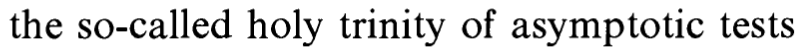
\includegraphics[scale=0.28]{figures/holy-trinity.png}
		\caption{A quote from \textcite[1229]{hausman-mcfadden-1984}.}
		\label{fig-holy-trinity}
	\end{figure}
	The \gls{lr} test/principle of testing was first proposed by \textcite{neyman-pearson-1928},
	and its asymptotic distribution was established by \textcite{wilks-1938}.
	\textcite{wald-1943} proposed the Wald test, and \textcite{rao-1948} proposed the score test,
	thereby completing the three classical large-sample tests.
	Their close asymptotic relationship was subsequently developed by \textcite{silvey-1959}.
	By the early 1980s, the three had acquired the rather grand name of the ``holy trinity'' of hypothesis testing.
	A quote shown in \autoref{fig-holy-trinity} attests to the reverence with which they are held.
\end{remark}

\vfill
\section*{Acronyms}
\printglossaries
\section*{References}
\printbibliography[heading=none]

\clearpage

\appendix
\section{Connection between \texorpdfstring{$F$}{F}-Test and Wald Test}\label{sec-f-test}

Consider the normal linear model
\begin{align}
	Y=X\beta+e,\qquad e\given X\sim\normaldistribution(0,\sigma^2 I_n),
\end{align}
where $X$ is $n\times k$ with full column rank and $n>k$.
To test $H_0:R\beta=r_0$, let $R$ be $q\times k$ with full row rank,
and let $\widehat\beta$ be the unrestricted \gls{ols} estimator.
Let $\widetilde\beta=\arg\min_{b:\,Rb=r_0}(Y-Xb)\T(Y-Xb)$ be the restricted estimator.
The two residual sums of squares are
\begin{align}
	\mathrm{RSS}_{\mathrm U}&=(Y-X\widehat\beta)\T(Y-X\widehat\beta),\\
	\mathrm{RSS}_{\mathrm R}&=(Y-X\widetilde\beta)\T(Y-X\widetilde\beta).
\end{align}
Set $s^2=\mathrm{RSS}_{\mathrm U}/(n-k)$.
The exact $F$-statistic is
\begin{align}
	T_F
	&=\frac{(R\widehat\beta-r_0)\T\big[R(X\T X)\inv R\T\big]\inv(R\widehat\beta-r_0)/q}{s^2}
	\sim F_{q,n-k}\quad\text{under }H_0,\label{eq-f-test}\\
	&=\frac{(\mathrm{RSS}_{\mathrm R}-\mathrm{RSS}_{\mathrm U})/q}{\mathrm{RSS}_{\mathrm U}/(n-k)}.
\end{align}
To see the second equality, the restricted normal equations give the explicit estimator
\begin{align}
	\widetilde\beta
	=\widehat\beta-(X\T X)\inv R\T\big[R(X\T X)\inv R\T\big]\inv(R\widehat\beta-r_0).
\end{align}
Since $Y-X\widetilde\beta=(Y-X\widehat\beta)+X(\widehat\beta-\widetilde\beta)$
and $X\T(Y-X\widehat\beta)=0$, expanding the squared residuals gives
\begin{align}
	\mathrm{RSS}_{\mathrm R}-\mathrm{RSS}_{\mathrm U}
	&=(\widehat\beta-\widetilde\beta)\T X\T X(\widehat\beta-\widetilde\beta)\\
	&=(R\widehat\beta-r_0)\T\big[R(X\T X)\inv R\T\big]\inv(R\widehat\beta-r_0).
\end{align}
Thus the numerator measures the increase in residual variation from imposing the null, per restriction.
The numerator in \eqref{eq-f-test}, before division by $q$, divided by $\sigma^2$ is $\chi_q^2$.
The denominator satisfies $(n-k)s^2/\sigma^2\sim\chi_{n-k}^2$ and is independent of that numerator, conditional on $X$.
This gives the exact $F$ distribution.
Using $\widehat V=n s^2(X\T X)\inv$ in the Wald statistic gives
\begin{align}
	T_{\mathrm W}=qT_F.
\end{align}
For fixed $q$, the denominator of an $F_{q,\nu}$ variable converges to one as $\nu\to\infty$.
Consequently,
\begin{align}
	T_t\sim t_\nu &\implies T_t\dto\normaldistribution(0,1),\\
	T_F\sim F_{q,\nu} &\implies qT_F\dto\chi_q^2.
\end{align}
These are the links between the finite-sample $t$ and $F$ tests and their asymptotic normal and Wald counterparts.
For a single restriction, $T_F=T_t^2$ exactly when both use the same $s^2$.

\begin{remark}[Heteroskedasticity]
	Use a robust covariance estimator $\widehat V$ in \eqref{eq-wald} when the errors are heteroskedastic.
	The resulting statistic still converges to $\chi_q^2$ under the appropriate moment and rank conditions,
	but dividing it by $q$ does not give an exact $F_{q,n-k}$ distribution.
	The residual-sum-of-squares formula above is not a robust test.
\end{remark}

\section{An Auxiliary Regression for the \texorpdfstring{\gls{lm}}{LM} Test}\label{sec-lm-auxiliary}

Consider the normal linear model
\begin{align*}
	Y=X_1\beta_1+X_2\beta_2+e,
	\qquad e\given X\sim\normaldistribution(0,\sigma^2 I_n),
\end{align*}
where $X=[X_1\;X_2]$ has full column rank and fewer columns than observations,
$X_1$ contains an intercept, and $X_2$ has $q$ columns.
We test $H_0:\beta_2=0$.
First regress $Y$ on $X_1$ only, obtaining restricted residuals
$\widetilde e=Y-X_1\widetilde\beta_1$ and the restricted variance estimate
$\widetilde\sigma^2=\widetilde e\T\widetilde e/n$.
Then run the \emph{auxiliary regression} of $\widetilde e$ on all the regressors $X=[X_1\;X_2]$.
Writing $P_X=X(X\T X)\inv X\T$, its fitted values are $P_X\widetilde e$.
Since the restricted regression includes an intercept, $\widetilde e$ has sample mean zero, so
\begin{align*}
	R_{\mathrm{aux}}^2
	=\frac{\widetilde e\T P_X\widetilde e}{\widetilde e\T\widetilde e}.
\end{align*}
To connect this to the score formula, write $\beta=(\beta_1\T,\beta_2\T)\T$.
The average coefficient score and its model-based information estimate are
\begin{align*}
	\frac{\partial\ell_n}{\partial\beta}(\widetilde\beta,\widetilde\sigma^2)
	=\frac{X\T\widetilde e}{n\widetilde\sigma^2},
	\qquad
	\widetilde I_{\beta\beta}=\frac{X\T X}{n\widetilde\sigma^2}.
\end{align*}
Here we use the conditional expected information evaluated at the restricted estimates;
its cross-block between $\beta$ and $\sigma^2$ is zero, and the variance score is zero at the restricted fit.
Thus \eqref{eq-lm} reduces to
\begin{align}
	T_{\mathrm{LM}}
	=\frac{\widetilde e\T P_X\widetilde e}{\widetilde\sigma^2}
	=nR_{\mathrm{aux}}^2
	\dto\chi_q^2\quad\text{under }H_0.
\end{align}
The intuition is simple: do the excluded regressors help explain what the restricted model leaves unexplained?
Although $X_1\T\widetilde e=0$, we retain $X_1$ in the auxiliary regression to control for its correlation with $X_2$.
This $nR^2$ formula uses the homoskedastic model; it is not automatically robust to heteroskedasticity.

\end{document}
